%%%%%%%%%%%%%%%%%%%%%%%%%%%%%%%%%%%%%%%%%%%%%%%%%%%%%%%%%%%
% --------------------------------------------------------
% Tau
% LaTeX Template
% Version 2.4.4 (28/02/2025)
%
% Author: 
% Guillermo Jimenez (memo.notess1@gmail.com)
% 
% License:
% Creative Commons CC BY 4.0
% --------------------------------------------------------
%%%%%%%%%%%%%%%%%%%%%%%%%%%%%%%%%%%%%%%%%%%%%%%%%%%%%%%%%%%

\documentclass[9pt,a4paper,twocolumn,twoside]{tau-class/tau}
\usepackage[brazil]{babel}

\usepackage{booktabs}
\usepackage{float}
\usepackage{graphicx}
\usepackage{siunitx}
\usepackage{tikz}
\usetikzlibrary{arrows.meta, positioning}

%% Spanish babel recomendation
% \usepackage[spanish,es-nodecimaldot,es-noindentfirst]{babel} 

%% Draft watermark
% \usepackage{draftwatermark}

%----------------------------------------------------------
% TITLE
%----------------------------------------------------------

\journalname{Relatório de Sistemas de Controle I - Etapa 1}
\title{Controle de Estabilização de um Pêndulo Invertido Rotacional}

%----------------------------------------------------------
% AUTHORS, AFFILIATIONS AND PROFESSOR
%----------------------------------------------------------

\author[a,1]{JOSÉ A. DA SILVA}
\author[b,2]{KAUA LESSA L. DOS SANTOS }
\author[c,3]{PABLO MUNIH S. DE CARVALHO}
\author[d,4]{PLÁCIDO AUGUSTUS DE O. CORDEIRO}

%----------------------------------------------------------

\affil[a]{Engenharia da Computação, Universidade Federal de Alagoas}
\affil[b]{Engenharia da Computação, Universidade Federal de Alagoas}
\affil[c]{Engenharia da Computação, Universidade Federal de Alagoas}

\professor{Prof. ICARO BEZERRA QUEIROZ DE ARAUJO}

%----------------------------------------------------------
% FOOTER INFORMATION
%----------------------------------------------------------

\institution{Universidade Federal de Alagoas}
%\footinfo{\LaTeX\ Template}%
\theday{\today}
% \leadauthor{Aluno et al.} %
\course{Engenharia da Computação}

%----------------------------------------------------------
% ABSTRACT AND KEYWORDS
%----------------------------------------------------------

\begin{abstract}    
    Este relatório trata da segunda etapa do projeto da disciplina de Sistemas de Controle I,
    de um pêndulo invertido rotacional. É apresentado, em primeira instância, as equações diferenciais
    de movimento do pêndulo obtidas através do método Euler-Lagrange \cite{ramos2011rotary}, 
    linearização do modelo e obtenção da função de transferência. Em seguida, a estabilidade do sistema é analisada, 
    assim como a resposta do modelo a diferentes entradas, a fim de prever seu comportamento. 
    Por fim, o software MATLAB/Simulink é utilizado para simular o sistema em malha aberta e os resultados são discutidos. 
\end{abstract}


%----------------------------------------------------------

\keywords{pêndulo invertido, controle rotacional, estabilização, sistemas não lineares}

%----------------------------------------------------------

\begin{document}
		
    \maketitle 
    \thispagestyle{firststyle} 
    \tauabstract 
    % \tableofcontents
    % \linenumbers 
    
%----------------------------------------------------------

\section{Introdução}
    \taustart{A}nteriormente, foi discutido a importância do pêndulo invertido no estudo prático de sistemas de controle, as
    diferenças entre os dois principais modelos presentes na literatura e a escolha do pêndulo invertido rotacional como
    interesse deste estudo.
    
    \subsection{Descrição do Sistema}
    Recapitulando, o pêndulo invertido rotacional, também chamado de Pêndulo de Furuta, é composto por um pêndulo acoplado
    a um braço horizontal giratório, que é acionado por um motor. O movimento do sistema ocorre no plano horizontal, através
    do movimento do braço giratório e no plano vertical, através do movimento do pêndulo. A relação de apenas um atuador para
    dois graus de liberdade caracteriza este sistema como subatuado. A Figura~\ref{fig:esquema} apresenta o modelo de 
    referência para a modelagem matemática e implementação do controlador. 

    \subsection{Variávies do Sistema}
    O sistema físico possui o torque do motor como única entrada. Para este estudo, apenas a ângulo do pêndulo será considerado
    como saída, dessa forma caracterizando um sistema \textit{single input single output} (SISO). É importante destacar
    que é possível considerar também o ângulo do braço como saída, dessa forma caracterizando um sistema
    \textit{single input multiple output} (SIMO), porém, esse não é o foco deste estudo. As variáveis físicas são
    apresentadas na tabela a seguir:

    \begin{table}[H]
    \centering
    \caption{Símbolos para descrever os parâmetros das equações}
    \begin{tabular}{ll}
        \toprule
        \textbf{Símbolo} & \textbf{Descrição} \\
        \midrule
        $L$   & Distância até o centro de massa do pêndulo \\
        $m$   & Massa do braço do pêndulo \\
        $r$   & Comprimento do braço rotativo \\
        $\theta$ & Ângulo do braço do pêndulo (rad) \\
        $\alpha$ & Ângulo do pêndulo (rad) \\
        $h$   & Distância do centro de massa do pêndulo até o solo \\
        $J_{cm}$ & Inércia do pêndulo em relação ao seu centro de massa \\
        $V_{x}$  & Velocidade do centro de massa do pêndulo na direção $x$ \\
        $V_{y}$  & Velocidade do centro de massa do pêndulo na direção $y$ \\
        \bottomrule
    \end{tabular}
\end{table}


\begin{figure}[H]
        \centering
        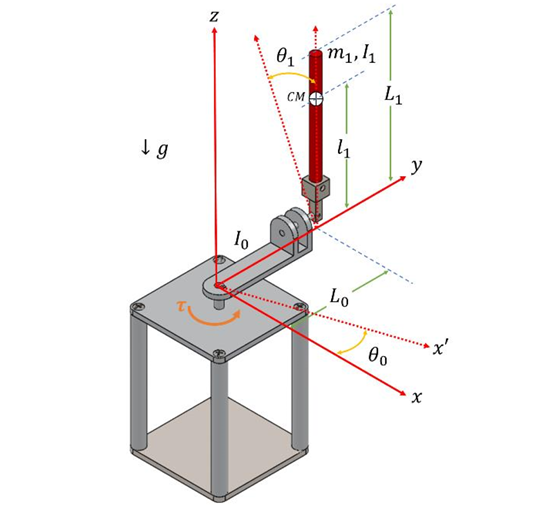
\includegraphics[width=0.85\columnwidth]{figures/pendulo com angulos.png}
        \caption{Representação tridimensional do pêndulo invertido rotacional com seus parâmetros físicos e coordenadas. Fonte: \cite{Duart2017}}
        \label{fig:esquema}
\end{figure} 

\subsection{Objetivo}
O objetivo desta etapa é a obtenção do modelo matemático que descreve a dinâmica do sistema, 
análisar o modelo obtido e simular através do software MATLAB/Simulink.

\section{Modelagem Matemática}

A compreensão precisa da dinâmica do Pêndulo de Furuta exige uma formulação matemática rigorosa. Antes de prosseguir com a derivação das equações de movimento, é fundamental estabelecer a convenção de coordenadas adotada. Conforme ilustrado na Figura~\ref{fig:angulo_pendulo}, o ângulo de rotação do braço horizontal é denotado por \(\theta\). O ponto crucial para a estabilização é a definição do ângulo \(\alpha\) do pêndulo em relação à vertical: o estado de interesse, onde o pêndulo se encontra na posição invertida (verticalmente para cima), corresponde explicitamente a \(\alpha = 0\). Essa definição é vital para a interpretação dos resultados de controle e para a linearização do sistema em torno deste ponto de equilíbrio instável.
A formulação adotada neste relatório segue de perto a apresentada em Ramos et al. \cite{ramos2011rotary}, 
que descrevem detalhadamente o procedimento de modelagem do pêndulo invertido rotacional (Pêndulo de Furuta). 
\begin{figure}[H]
    \centering
    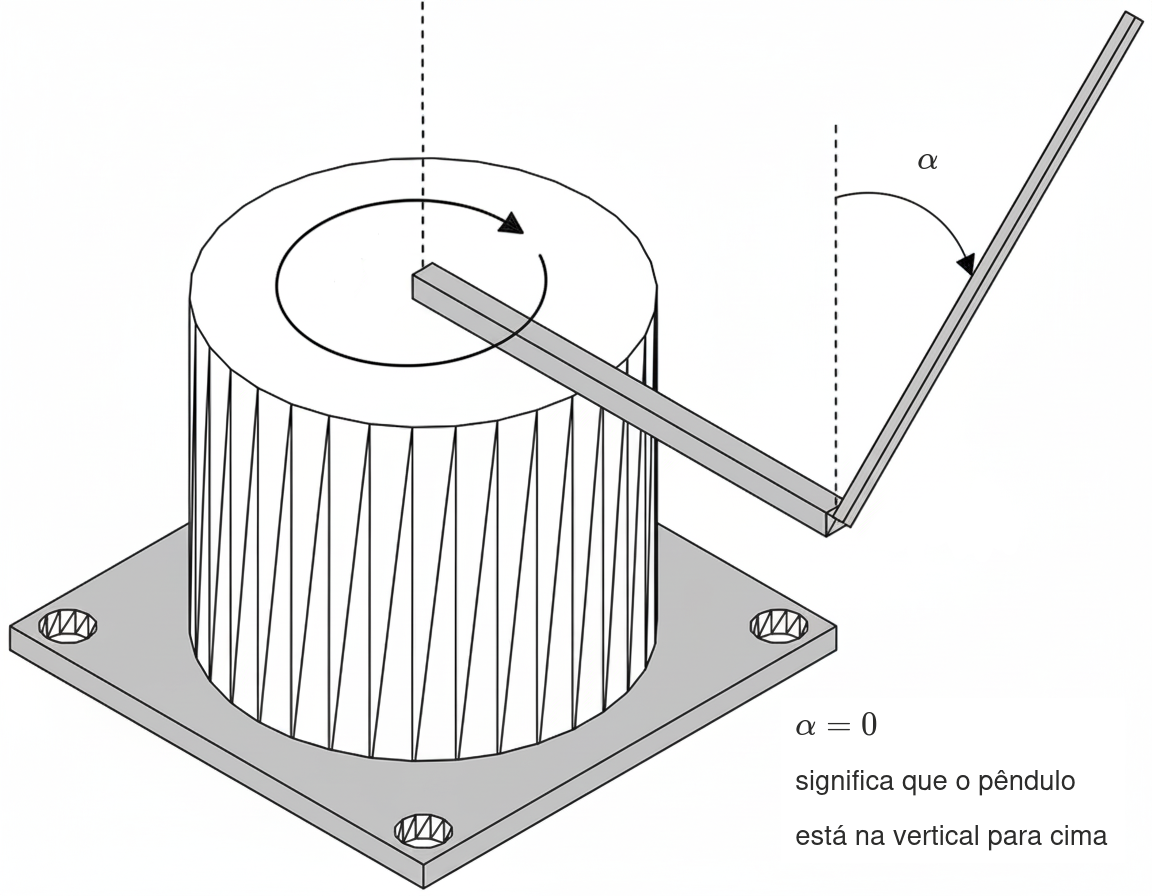
\includegraphics[width=0.9\columnwidth]{figures/angulo_pendulo.png} % Ajustado para columnwidth
    \caption{Definição das variáveis angulares do Pêndulo de Furuta, com o ângulo do braço \(\theta\) e o ângulo do pêndulo \(\alpha\). A posição de equilíbrio instável (\(\alpha=0\)) é indicada.}
    \label{fig:angulo_pendulo}
\end{figure}

A modelagem matemática do pêndulo invertido rotacional é obtida aplicando o 
método de Euler-Lagrange. Inicialmente, consideram-se as velocidades do 
centro de massa do pêndulo e do braço rotativo:

\begin{equation}
    V_{Pen.\,cm} = -L \cos (\alpha) \, \dot{\alpha} \, \hat{x} - L \sin (\alpha) \, \dot{\alpha} \, \hat{y}
\end{equation}

\begin{equation}
    V_{arm} = r \dot{\theta}
\end{equation}

Assim, as componentes de velocidade do centro de massa do pêndulo podem ser escritas como:
\begin{align}
    V_x &= r\dot{\theta} - L\cos(\alpha) \, \dot{\alpha} \\
    V_y &= -L\sin(\alpha) \, \dot{\alpha}
\end{align}

\subsection{Energia Potencial}
A única energia potencial no sistema é a gravitacional:
\begin{equation}
    V = m g h = m g L \cos(\alpha)
\end{equation}

\subsection{Energia Cinética}
As energias cinéticas são devidas ao movimento do braço, ao movimento do centro 
de massa do pêndulo e à rotação do pêndulo em torno do seu próprio centro de massa:

\begin{equation}
    T = KE_{hub} + KE_{V_x} + KE_{V_y} + KE_{pendulo}
\end{equation}

\subsubsection*{Momento de Inércia}
O momento de inércia de uma barra homogênea em torno do centro de massa é:
\begin{equation}
    J_{cm} = \frac{1}{12} M R^2
\end{equation}
Como o comprimento do pêndulo é $2L$, temos:
\begin{equation}
    J_{cm} = \frac{1}{12} M (2L)^2 = \frac{1}{3} M L^2
\end{equation}

\subsubsection*{Energia Cinética do Braço (Hub)}
\begin{equation}
    T_{hub} = \tfrac{1}{2} J_{eq} \dot{\theta}^2
\end{equation}

\subsubsection*{Energia Cinética de Translação do Pêndulo}
\begin{equation}
    T_{trans} = \tfrac{1}{2} m (V_x^2 + V_y^2)
\end{equation}
Substituindo as velocidades:
\begin{equation}
    T_{trans} = \tfrac{1}{2} m \Big[ (r \dot{\theta} - L \cos(\alpha) \, \dot{\alpha})^2 + (-L \sin(\alpha) \, \dot{\alpha})^2 \Big]
\end{equation}

\subsubsection*{Energia Cinética de Rotação do Pêndulo em torno do CM}
\begin{equation}
    T_{rot} = \tfrac{1}{2} J_{cm} \dot{\alpha}^2
\end{equation}

\subsubsection*{Energia Cinética Total}

Somando todas as parcelas de energia cinética, temos:
\begin{equation}
    T = \tfrac{1}{2} J_{eq} \dot{\theta}^2 
        + \tfrac{1}{2} m (r \dot{\theta} - L \cos(\alpha) \dot{\alpha})^2
        + \tfrac{1}{2} m (-L \sin(\alpha) \dot{\alpha})^2
        + \tfrac{1}{2} J_{cm} \dot{\alpha}^2
    \label{eq:Ttotal1}
\end{equation}

Expandindo os quadrados:
\begin{align}
    T &= \tfrac{1}{2} J_{eq} \dot{\theta}^2 
        + \tfrac{1}{2} m \big(r^2 \dot{\theta}^2 - 2 r L \cos(\alpha) \, \dot{\theta}\dot{\alpha} + L^2 \cos^2(\alpha) \, \dot{\alpha}^2 \big) \nonumber \\
      &\quad + \tfrac{1}{2} m \big(L^2 \sin^2(\alpha) \, \dot{\alpha}^2\big)
        + \tfrac{1}{2} \Big(\tfrac{1}{3} m L^2\Big) \dot{\alpha}^2
    \label{eq:Ttotal2}
\end{align}

Reagrupando os termos:
\begin{align}
    T &= \tfrac{1}{2}(J_{eq} + m r^2) \dot{\theta}^2 
        - m L r \cos(\alpha) \, \dot{\theta}\dot{\alpha} \nonumber \\
      &\quad + \tfrac{1}{2} m L^2 (\cos^2(\alpha) + \sin^2(\alpha))\dot{\alpha}^2
        + \tfrac{1}{6} m L^2 \dot{\alpha}^2
    \label{eq:Ttotal3}
\end{align}

Como $\cos^2(\alpha) + \sin^2(\alpha) = 1$, temos:
\begin{equation}
    T = \tfrac{1}{2}(J_{eq} + m r^2) \dot{\theta}^2 
        - m L r \cos(\alpha) \, \dot{\theta}\dot{\alpha} 
        + \tfrac{2}{3} m L^2 \dot{\alpha}^2
    \label{eq:TtotalFinal}
\end{equation}


\subsection{Lagrangiana}

A energia potencial e a energia cinética total foram obtidas como:
\begin{align}
    V &= m g L \cos(\alpha) \\
    T &= \tfrac{1}{2}(J_{eq} + m r^2)\dot{\theta}^2 
        - m L r \cos(\alpha)\,\dot{\theta}\dot{\alpha}
        + \tfrac{2}{3} m L^2 \dot{\alpha}^2
\end{align}

Portanto, a Lagrangiana é:
\begin{equation}
    \mathcal{L} = T - V
\end{equation}

\begin{equation}
    \mathcal{L} = \tfrac{1}{2}(J_{eq} + m r^2)\dot{\theta}^2
        - m L r \cos(\alpha)\,\dot{\theta}\dot{\alpha}
        + \tfrac{2}{3} m L^2 \dot{\alpha}^2
        - m g L \cos(\alpha)
\end{equation}

\subsection{Equações de Lagrange}

A equação de Lagrange geral para uma coordenada generalizada $q_i$ é:
\begin{equation}
    \frac{d}{dt}\left(\frac{\partial \mathcal{L}}{\partial \dot{q}_i}\right)
    - \frac{\partial \mathcal{L}}{\partial q_i} = Q_i
\end{equation}

No sistema, temos as duas coordenadas generalizadas:
\[
q_1 = \theta, \qquad q_2 = \alpha
\]



\subsubsection*{Para $\theta$}
\begin{equation}
    \frac{d}{dt}\left(\frac{\partial \mathcal{L}}{\partial \dot{\theta}}\right)
    - \frac{\partial \mathcal{L}}{\partial \theta}
    = T_{output} - B_{eq}\dot{\theta}
\end{equation}

- A coordenada $\theta$ recebe o torque do motor. 

- Esse torque possui duas partes:

    1. $T_{output}$: torque útil gerado pelo motor.  

    2. $-B_{eq}\dot{\theta}$: torque dissipativo devido ao atrito viscoso.  



\subsubsection*{Aplicando a $\alpha$}

Para a coordenada $\alpha$, a equação de Lagrange é:
\begin{equation}
    \frac{d}{dt}\left(\frac{\partial \mathcal{L}}{\partial \dot{\alpha}}\right)
    - \frac{\partial \mathcal{L}}{\partial \alpha} = 0
\end{equation}

\noindent
Observações importantes:
\begin{itemize}
    \item A coordenada $\alpha$ não recebe torque aplicado diretamente.
    \item O único efeito externo é a gravidade (já incluída na energia potencial).
    \item Por isso, o lado direito da equação é nulo.
\end{itemize}



\subsubsection*{Equações diferenciais finais}

Após aplicar as equações de Lagrange para $\theta$ e $\alpha$, e linearizar em torno de $\alpha \approx 0$, obtemos:

\begin{align}
    (J_{eq} + m r^2)\ddot{\theta} - m L r \ddot{\alpha} &= T_{output} - B_{eq}\dot{\theta} 
    && \text{(Braço)} \\
    \tfrac{4}{3} m L^2 \ddot{\alpha} - m L r \ddot{\theta} - m g L \alpha &= 0
    && \text{(Pêndulo)}
\end{align}



\subsection{Modelo em Espaço de Estados}

O torque de saída do motor aplicado ao sistema é dado por:
\begin{equation}
    T_{output} = \frac{\eta_m \eta_g K_t K_g}{R_m} \left( V_m - K_G K_m \dot{\theta} \right) 
    \label{eq:torque}
\end{equation}

Combinando as equações de movimento obtidas, a representação em espaço de estados pode ser escrita como:
\begin{equation}
\begin{bmatrix}
\dot{\theta} \\
\dot{\alpha} \\
\ddot{\theta} \\
\ddot{\alpha}
\end{bmatrix}
=
\begin{bmatrix}
0 & 0 & 1 & 0 \\
0 & 0 & 0 & 1 \\
0 & \tfrac{bd}{E} & -\tfrac{cG}{E} & 0 \\
0 & \tfrac{qd}{E} & -\tfrac{bG}{E} & 0
\end{bmatrix}
\begin{bmatrix}
\theta \\ \alpha \\ \dot{\theta} \\ \dot{\alpha}
\end{bmatrix}
+
\begin{bmatrix}
0 \\
0 \\
\tfrac{c \, \eta_m \eta_g K_t K_g}{R_m E} \\
\tfrac{b \, \eta_m \eta_g K_t K_g}{R_m E}
\end{bmatrix} V_m
\label{eq:estado}
\end{equation}

onde os parâmetros são definidos como:
\begin{align*}
a &= J_{eq} + mr^2, & b &= mLr, \\
c &= \tfrac{4}{3} mL^2, & d &= mgL, \\
E &= ac - b^2, & G &= \tfrac{\eta_m \eta_g K_t K_m K_g^2}{R_m} - B_{eq}
\end{align*}

A Tabela~\ref{tab:parametros} apresenta os parâmetros utilizados para o sistema SRV02.

\begin{table}[H]
\centering
\caption{Parâmetros típicos do sistema SRV02 e do pêndulo}
\label{tab:parametros}
\begin{tabular}{lll}
\toprule
\textbf{Símbolo} & \textbf{Descrição} & \textbf{Valor} \\
\midrule
$K_t$   & Constante de torque do motor            & 0.00767 \\
$K_m$   & Constante de FEM inversa                & 0.00767 \\
$R_m$   & Resistência de armadura                 & 2.6 \\
$K_g$   & Relação de engrenagem (motor $\rightarrow$ carga) & 14 (14:1) \\
$\eta_m$ & Eficiência do motor                    & 0.69 \\
$\eta_g$ & Eficiência da caixa de engrenagem      & 0.9 \\
$B_{eq}$ & Coef. de atrito viscoso equivalente    & $1.5 \times 10^{-3}$ \\
$J_{eq}$ & Momento de inércia equivalente na carga & $9.31 \times 10^{-4}$ \\
\bottomrule
\end{tabular}
\end{table}

\subsection{Modelo Numérico em Espaço de Estados}

Substituindo os valores da Tabela~\ref{tab:parametros}, obtemos o modelo em espaço de estados numérico:

\begin{equation}
\begin{bmatrix}
\dot{\theta} \\
\dot{\alpha} \\
\ddot{\theta} \\
\ddot{\alpha}
\end{bmatrix}
=
\begin{bmatrix}
0 & 0 & 1 & 0 \\
0 & 0 & 0 & 1 \\
0 & 39.32 & -14.52 & 0 \\
0 & 81.78 & -13.98 & 0
\end{bmatrix}
\begin{bmatrix}
\theta \\ \alpha \\ \dot{\theta} \\ \dot{\alpha}
\end{bmatrix}
+
\begin{bmatrix}
0 \\ 0 \\ 25.54 \\ 24.59
\end{bmatrix} V_m
\label{eq:estadoNum}
\end{equation}

E a saída é dada por:
\begin{equation}
Y =
\begin{bmatrix}
1 & 0 & 0 & 0 \\
0 & 1 & 0 & 0
\end{bmatrix}
\begin{bmatrix}
\theta \\ \alpha \\ 
\end{bmatrix}
+
\begin{bmatrix}
0 \\ 0
\end{bmatrix} V_m
\end{equation}

\subsection{Obtenção da Função de Transferência}

A partir do modelo em espaço de estados (Eq.~\ref{eq:estadoNum}), pode-se obter a 
função de transferência que relaciona a entrada do sistema (tensão no motor $V_m$) 
com a saída escolhida (ângulo do pêndulo $\alpha$). Para isso, foi utilizada a 
função \texttt{tf()} do \textit{MATLAB}, que converte a representação em espaço 
de estados para a forma de função de transferência.

As matrizes do sistema são definidas como:

\begin{equation}
\begin{split}
A &=
\begin{bmatrix}
0 & 0 & 1 & 0 \\
0 & 0 & 0 & 1 \\
0 & 39.32 & -14.52 & 0 \\
0 & 81.78 & -13.98 & 0
\end{bmatrix}, \quad
B =
\begin{bmatrix}
0 \\ 0 \\ 25.54 \\ 24.59
\end{bmatrix}, \\
C &= 
\begin{bmatrix}
0 & 1 & 0 & 0
\end{bmatrix}, \quad
D = 0
\end{split}
\end{equation}

O código em \textit{MATLAB} para a conversão é o seguinte:

\begin{verbatim}
A = [0 0 1 0;
     0 0 0 1;
     0 39.32 -14.52 0;
     0 81.78 -13.98 0];

B = [0; 0; 25.54; 24.59];

C = [0 1 0 0];   % Saída = ângulo do pêndulo
D = 0;

sys_ss = ss(A, B, C, D);  % Espaço de estados
sys_tf = tf(sys_ss);      % Função de transferência
\end{verbatim}

Assim, obtém-se diretamente a função de transferência $G(s)$, que expressa a 
dinâmica do sistema:

\begin{equation}
    G(s) = \frac{\alpha(s)}{V_m(s)}
          = \frac{24.59\,s - 0.0024}{s^3 + 14.52\,s^2 - 81.78\,s - 637.8}
\end{equation}

onde $\alpha(s)$ é a transformada de Laplace do ângulo do pêndulo e $V_m(s)$ é a 
transformada de Laplace da tensão aplicada ao motor.


\begin{figure}[H]
    \centering
    \begin{tikzpicture}[auto, node distance=2cm, >=Latex]
        \node [draw, rectangle, minimum width=3.5cm, minimum height=1cm, align=center] (plant) 
        {$G(s) = \dfrac{\alpha(s)}{V_m(s)}$};
        \node [left=of plant] (input) {$V_m(s)$};
        \node [right=of plant] (output) {$\alpha(s)$};
        \draw [->] (input) -- (plant);
        \draw [->] (plant) -- (output);
    \end{tikzpicture}
    \caption{Diagrama de blocos representando a função de transferência entre a entrada $V_m(s)$ e a saída $\alpha(s)$.}
    \label{fig:tf_pendulo}
\end{figure}




\section{Análise do Modelo}
Após a obtenção da função de transferência que descreve a dinâmica entre a entrada $V_m(s)$ (tensão aplicada ao motor) e a saída $\alpha(s)$ (ângulo do pêndulo), procede-se à análise matemática do sistema em malha aberta. Essa análise permite caracterizar propriedades fundamentais, como ordem e grau relativo, localização dos polos e zeros, estabilidade intrínseca e comportamento esperado diante de diferentes entradas. Embora ainda não haja controle implementado, esta etapa é essencial para compreender as limitações naturais do sistema e justificar a necessidade de técnicas de estabilização.
\subsection{Ordem e grau relativo}
\begin{itemize}
    \item \textbf{Ordem do sistema:} 3 (denominador de grau 3) — sistema de 3ª ordem.
    \item \textbf{Grau do numerador:} 1.
\end{itemize}

\subsection{Polos e estabilidade}
As raízes do denominador (polos) obtidos numericamente são aproximadamente:
\[
p_1 \approx -17.12,\qquad p_2 \approx -4.94,\qquad p_3 \approx +7.54.
\]
Como existe um polo em \(\,p_3 \approx +7.54\) (semiplano direito), o sistema é \textbf{instável em malha aberta}. Em termos práticos, qualquer pequena perturbação tenderá a crescer exponencialmente se não houver controle.
A raiz do numerador (zero) é aproximadamente:
\[
z \approx +9.76\times 10^{-5}.
\]

\begin{figure}[H]
    \centering
    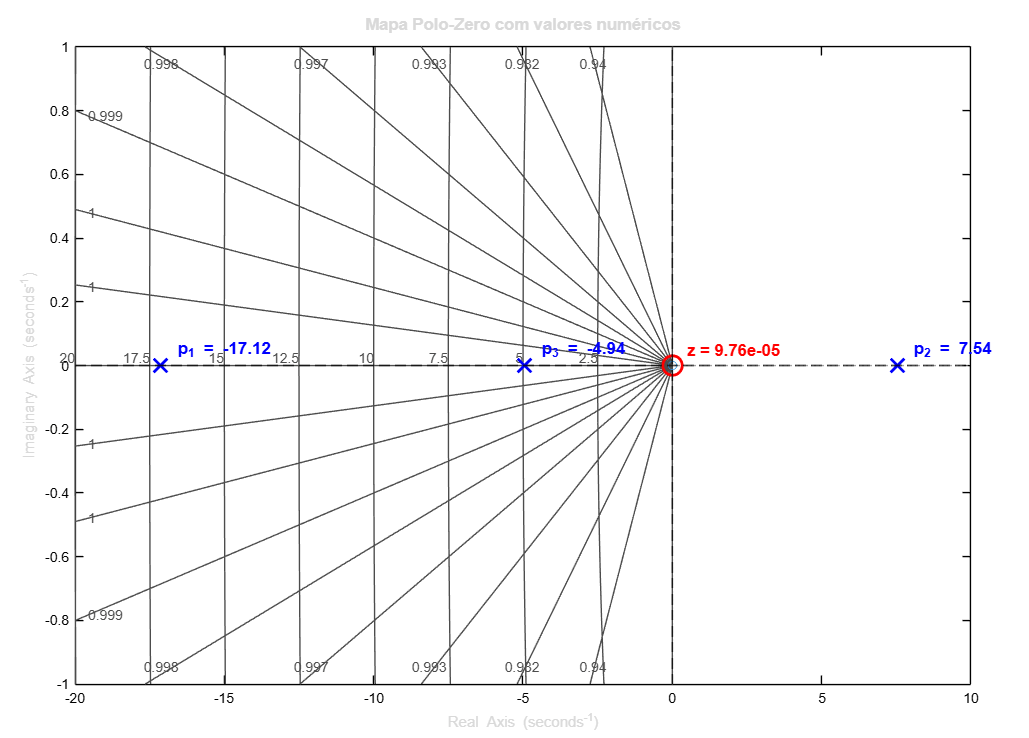
\includegraphics[width=\columnwidth]{figures/polos_e_zeros.png}
    \caption{Mapa polo-zero do sistema, com polos (X) e zeros (O) destacados numericamente.}
    \label{fig:pzmap}
\end{figure}

O sistema possui, portanto, um zero no semiplano direito (RHP), caracterizando-o como \textbf{não mínimo-fase}, a principal consequência disso é a tendência do sistema de apresentar uma resposta inversa (\textit{undershoot}). Se o sistema fosse estável e recebesse um comando em degrau para ir a um valor positivo, a saída primeiro se moveria ligeiramente na direção negativa antes de se corrigir.

\subsection{Ganho DC}
O ganho estático do sistema é:
\[
G(0)=\frac{-0.0024}{-637.752}\approx 3.76\times 10^{-6}.
\]
O valor é muito pequeno, mas na prática a dinâmica é dominada pelo polo instável.

\subsection{Tipo do sistema}
Não há polos em $s=0$, logo o sistema é do \textbf{tipo 0}. Em teoria isso significa erro finito para entrada em degrau, mas devido à instabilidade, em malha aberta a saída tende a divergir.

\subsection{Observações finais}
\begin{itemize}
    \item O polo no semiplano direito torna o sistema instável em malha aberta.
    \item O zero no semiplano direito impõe dificuldades na modelagem de um controlador 
\end{itemize}

\section{Simulação Computacional}
Para validar e visualizar o comportamento dinâmico previsto pela análise matemática, o sistema foi simulado no ambiente \textit{MATLAB/Simulink}. Utilizando a função de transferência \(G(s)\) obtida, foram analisadas as respostas do sistema em malha aberta a três sinais de entrada canônicos: impulso, degrau e rampa. Essas simulações são fundamentais para confirmar a instabilidade inerente do pêndulo e compreender a natureza da sua resposta antes da implementação de qualquer estratégia de controle. O comportamento observado em todas as simulações reflete diretamente a presença do polo instável em \(s \approx +7.54\).

\subsection{Resposta ao Impulso}
A resposta a um impulso unitário, que representa a reação do sistema a uma perturbação instantânea de energia, é apresentada na Figura~\ref{fig:impulse}. Como se pode observar, a saída (ângulo do pêndulo) diverge exponencialmente, confirmando a instabilidade do sistema em malha aberta. Uma perturbação mínima é suficiente para que o pêndulo inicie um movimento de queda do qual ele não consegue se recuperar autonomamente. Esse comportamento é totalmente consistente com o polo no semiplano direito, que domina a dinâmica do sistema.

\begin{figure}[H]
    \centering
    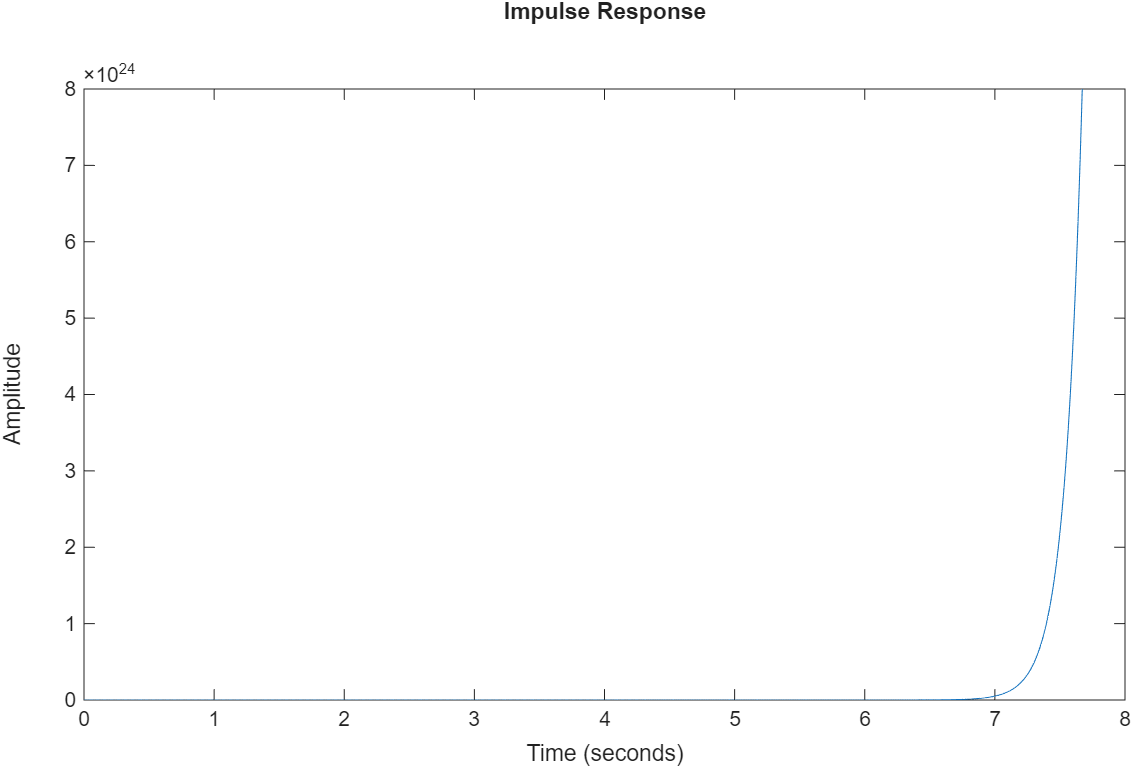
\includegraphics[width=0.45\textwidth]{figures/impulse_response.png}
    \caption{Resposta ao impulso do sistema em malha aberta.}
    \label{fig:impulse}
\end{figure}

\subsection{Resposta ao Degrau}
A aplicação de uma entrada em degrau, que equivale a fornecer uma tensão constante ao motor, também resulta em uma resposta instável, como ilustrado na Figura~\ref{fig:step}. A saída cresce de forma ilimitada, o que, fisicamente, corresponde à queda do pêndulo de forma acelerada. O resultado reforça que uma ação de controle constante é incapaz de estabilizar o sistema, evidenciando a necessidade de uma malha de realimentação que ajuste a entrada dinamicamente com base no estado do pêndulo.

\begin{figure}[H]
    \centering
    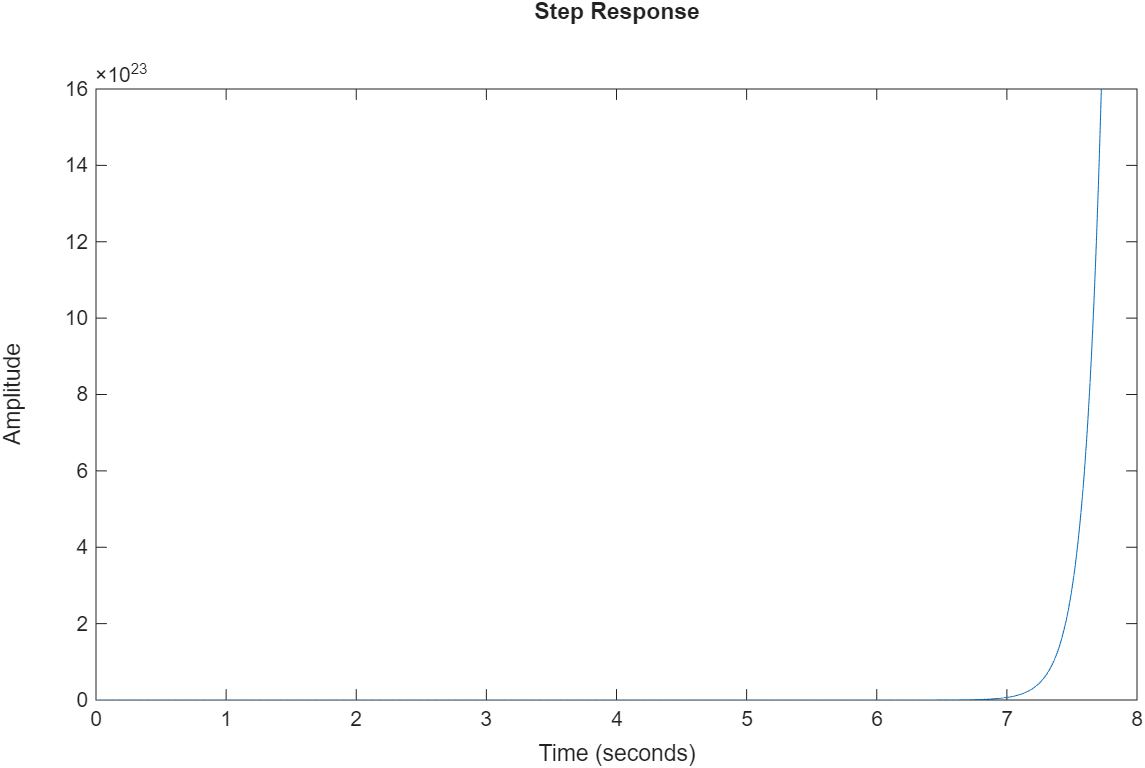
\includegraphics[width=0.45\textwidth]{figures/step_response.png}
    \caption{Resposta ao degrau do sistema em malha aberta.}
    \label{fig:step}
\end{figure}

\subsection{Resposta à Rampa}
A resposta a uma entrada do tipo rampa, mostrada na Figura~\ref{fig:ramp}, exibe uma divergência ainda mais acentuada. Este teste submete o sistema a uma solicitação de energia continuamente crescente, e a resposta instável se manifesta de forma mais rápida e agressiva. Embora seja um cenário menos comum na prática, a simulação confirma que o sistema em malha aberta é incapaz de seguir qualquer trajetória de referência, por mais simples que seja, reforçando a necessidade crítica de um controlador para a estabilização.

\begin{figure}[H]
    \centering
    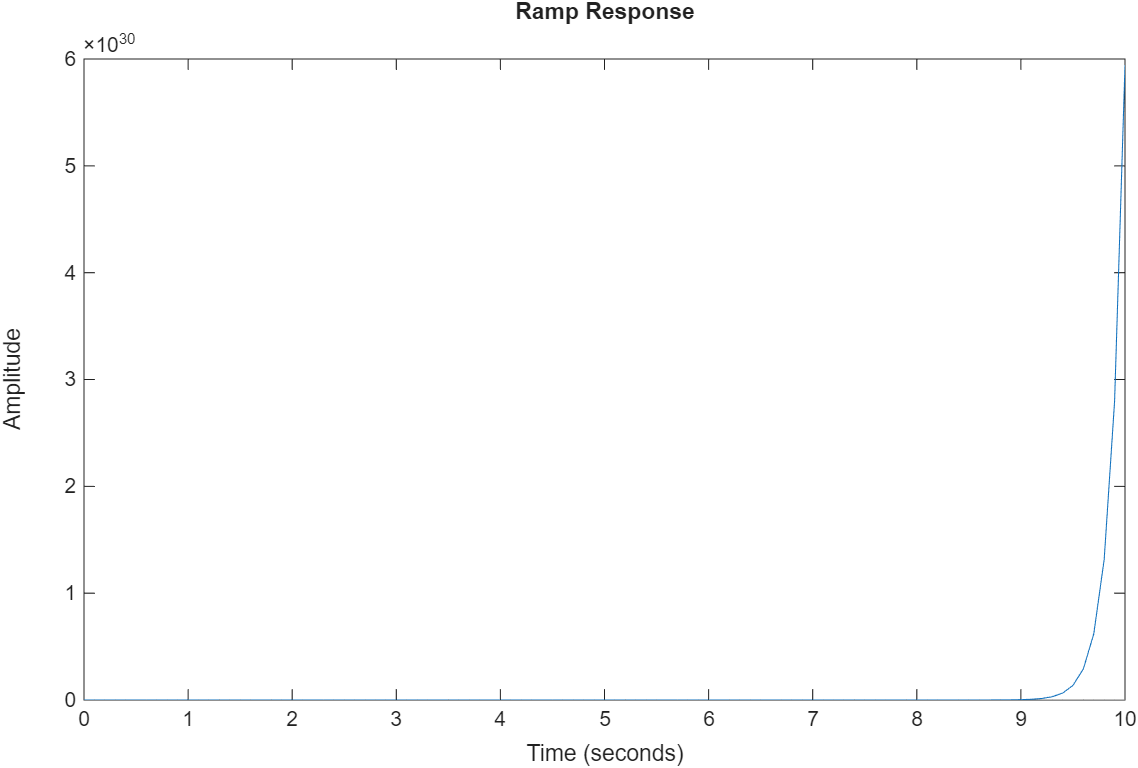
\includegraphics[width=0.45\textwidth]{figures/ramp_response.png}
    \caption{Resposta à rampa do sistema em malha aberta.}
    \label{fig:ramp}
\end{figure}

\section{Conclusão}
Nesta etapa do projeto, o modelo matemático para o pêndulo invertido rotacional (Pêndulo de Furuta) foi obtido com sucesso. Partindo dos princípios da mecânica clássica e utilizando o método de Euler-Lagrange, foram derivadas as equações diferenciais não lineares que descrevem a dinâmica do sistema. Subsequentemente, o modelo foi linearizado em torno do ponto de equilíbrio instável (\(\alpha \approx 0\)) para se obter uma representação em espaço de estados e a correspondente função de transferência, relacionando a tensão de entrada do motor (\(V_m\)) com o ângulo do pêndulo (\(\alpha\)).

A análise da função de transferência revelou características cruciais do sistema em malha aberta. Foi identificado que o sistema é de terceira ordem, do tipo 0, e, mais importante, intrinsecamente instável devido a um polo localizado no semiplano direito (\(p_3 \approx +7.54\)). Adicionalmente, a presença de um zero também no semiplano direito caracteriza o sistema como de fase não mínima, o que pode impor desafios ao projeto do controlador, como a ocorrência de uma resposta inversa inicial (\textit{undershoot}).

As simulações computacionais do sistema em malha aberta para entradas de impulso, degrau e rampa confirmaram visualmente a instabilidade prevista pela análise teórica, com a saída divergindo exponencialmente em todos os cenários. Os resultados obtidos nesta etapa concluem a modelagem e a análise do sistema, fornecendo uma base sólida e indispensável para a próxima fase do projeto. A próxima etapa consistirá no projeto e implementação de um controlador em malha fechada com o objetivo de superar a instabilidade natural do sistema e manter o pêndulo estabilizado na posição vertical.

    % \begin{itemize}
    %     \item BREGANON, R. et al. Desenvolvimento de sistemas de pêndulos invertidos como ferramentas didáticas em cursos de engenharia de controle e automação. \textit{HOLOS}, v. 7, p. 1–14, 2021. DOI: 10.15628/holos.2021.10351.
    
    %     \item DUART, J. L. et al. Dynamic modeling and simulation of a rotational inverted pendulum. \textit{Journal of Physics: Conference Series}, v. 792, 2017.
    
    %     \item CASAS, V. M. et al. Construção e projeto de controle de um protótipo de pêndulo invertido rotacional. \textit{EasyChair Preprint}, 2024.
    
    %     \item JAKOBSSON, S. Á. Control of a rotary inverted pendulum system using computer vision. Master’s Thesis – Reykjavik University, 2024.
    
    %     \item YAMANE, L. de S. Projeto mecânico e síntese do controlador de um pêndulo de Furuta. Trabalho de Conclusão de Curso (Engenharia Mecânica) – Universidade Federal do Amazonas, 2020.
    % \end{itemize}


%----------------------------------------------------------
% \nocite{yamane2021}
\printbibliography

%----------------------------------------------------------

\end{document}